\chapter{DApp design and implementation} 
\label{chapter:introduction}

\section{User Registration \& Sign in}
\begin{figure}[htb]
    \centering
    \frame{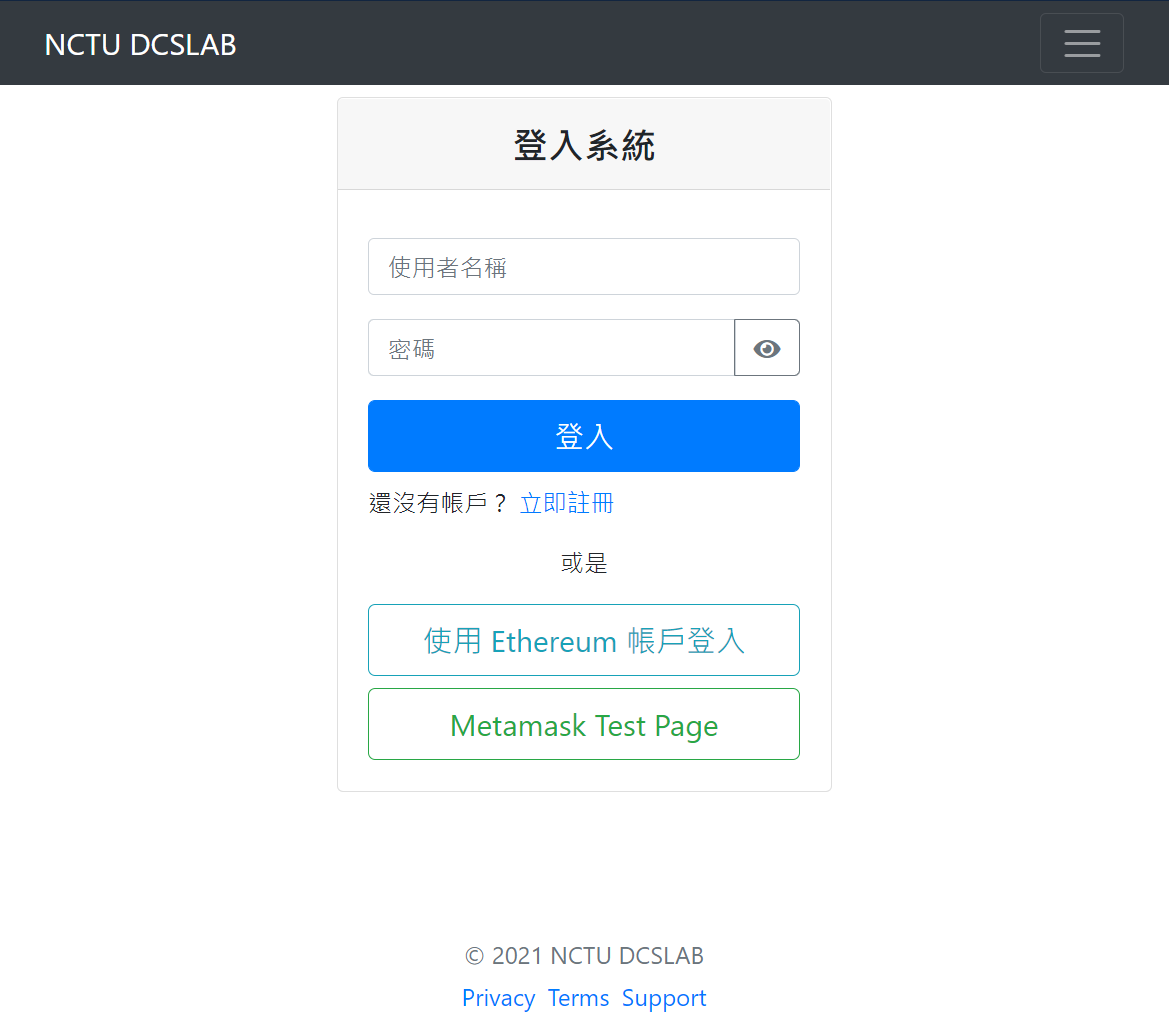
\includegraphics[height=!,width=0.8\linewidth,keepaspectratio=true]{figures/screenshot_signin.png}}
    \caption{{\footnotesize Screenshot of sign in page}}
    \label{fig:signin}
\end{figure}

A user in our proposed system must register as a member of any \(Orgs\) and provider his identification number as indicated in the Figure~\ref{fig:signup}. Afterwards, if the user wants to activate the third-party login, he submits a binding request after the login. As shown in the Figure~\ref{fig:signinblockchain} below, the user clicks on the "Login with Ethereum account" button and the MetaMask signature request will appear to ask the user for confirmation. The purpose of this step is to ensure that the user has ownership of the Ethereum account.
\begin{figure}[h]
    \centering
    \frame{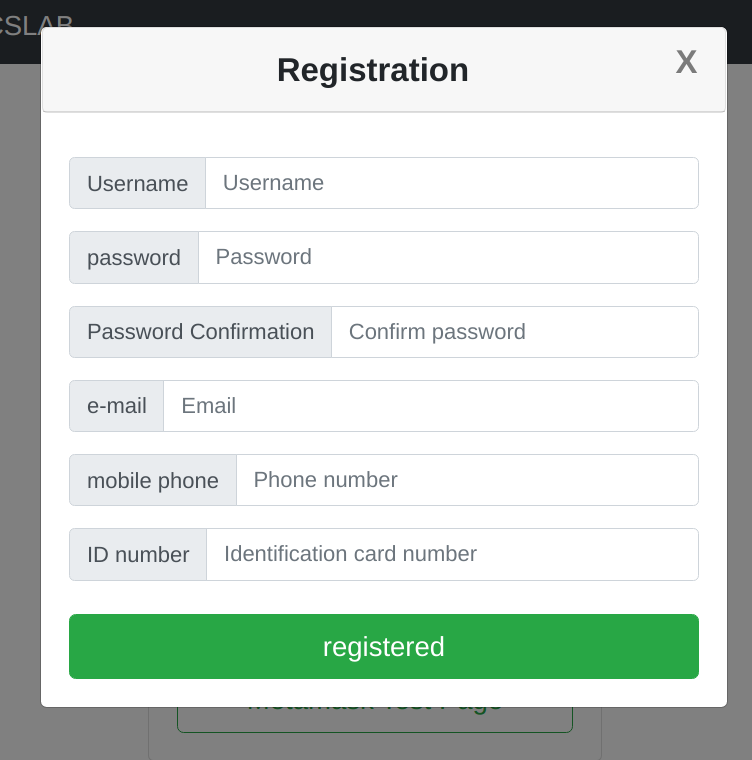
\includegraphics[height=!,width=0.75\linewidth,keepaspectratio=true]{figures/screenshot_signup.png}}
    \caption{{\footnotesize Screenshot of sign up window}}
    \label{fig:signup}
\end{figure}

\begin{figure}[h]
    \centering
    \frame{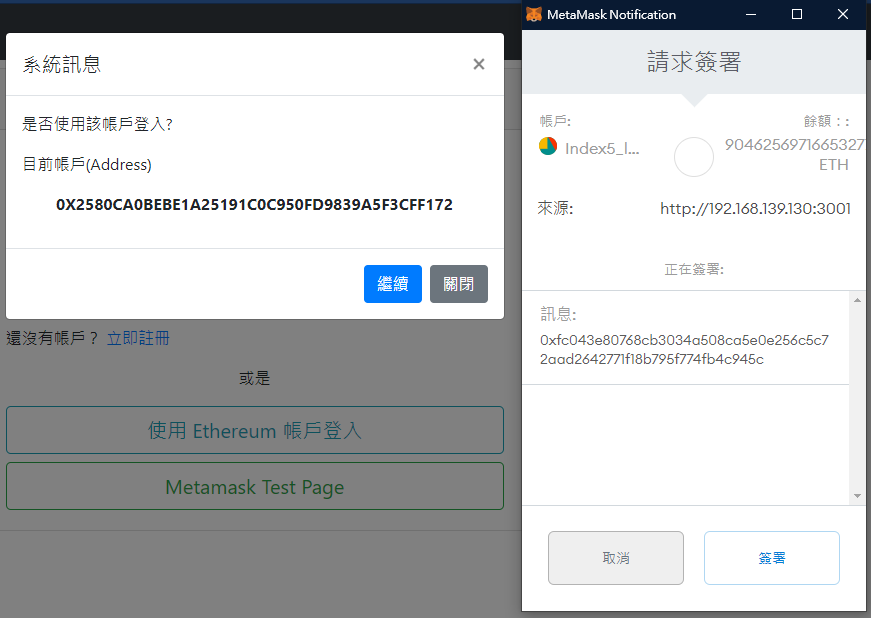
\includegraphics[height=!,width=0.75\linewidth,keepaspectratio=true]{figures/screenshot_thirdpartysignin.png}}
    \caption{{\footnotesize Screenshot of sign in with blockchain}}
    \label{fig:signinblockchain}
\end{figure}
\clearpage
\newpage

\section{User's Profile}

\begin{figure}[htb]
    \centering
    \frame{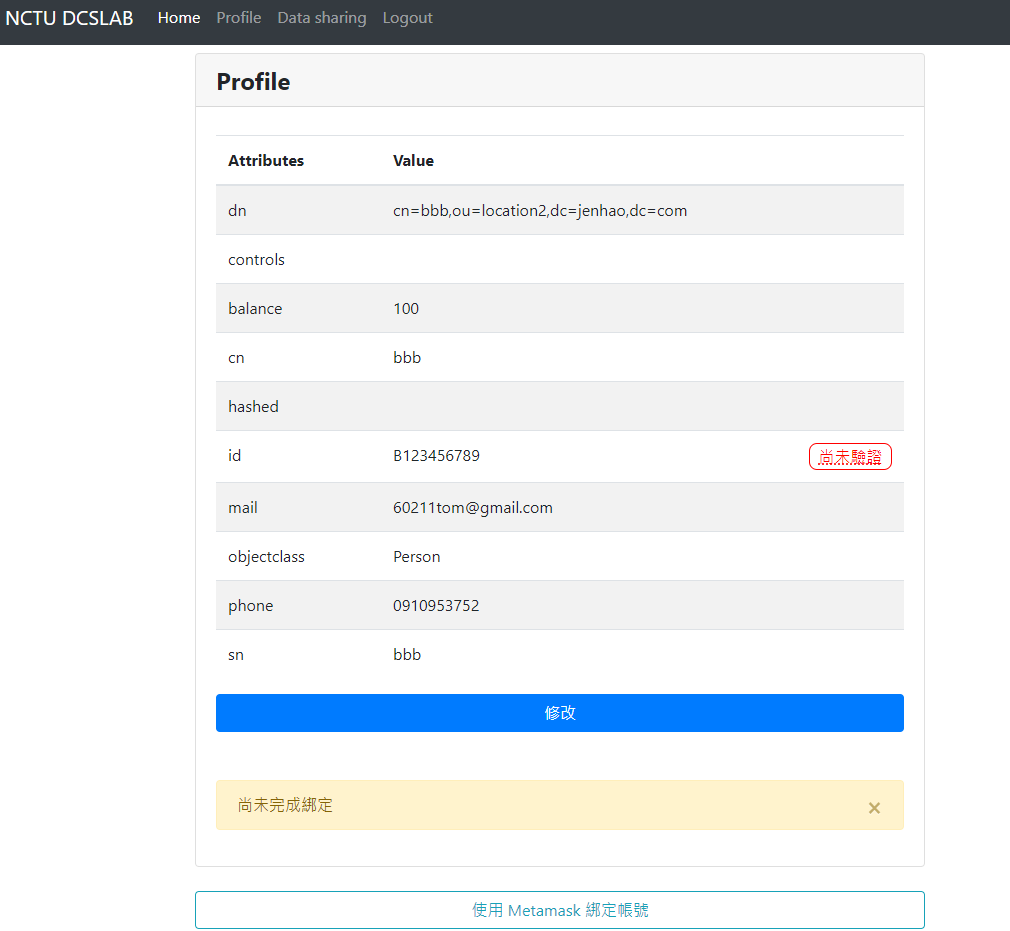
\includegraphics[height=!,width=0.9\linewidth,keepaspectratio=true]{figures/screenshot_profile.png}}
    \caption{{\footnotesize Screenshot of user's profile}}
    \label{fig:profile}
\end{figure}
After the user log in to the Org's service, the user can view their own full profile. Since our implementation adopted the Lightweight Directory Access Protocol (LDAP) to authenticate users, it has stored and retrieved user information from a hierarchical directory structure. As shown in Figure~\ref{fig:profile}, these attributes are parts of the X.500 directory specification, which defines nodes in an LDAP directory. E.g., \textit{dn} (distinguished name), \textit{cn} (common name). In this paper, we also define custom attributes such as \textit{balance}, \textit{hashed}.
\newpage

\begin{figure}[htb]
    \centering
    \frame{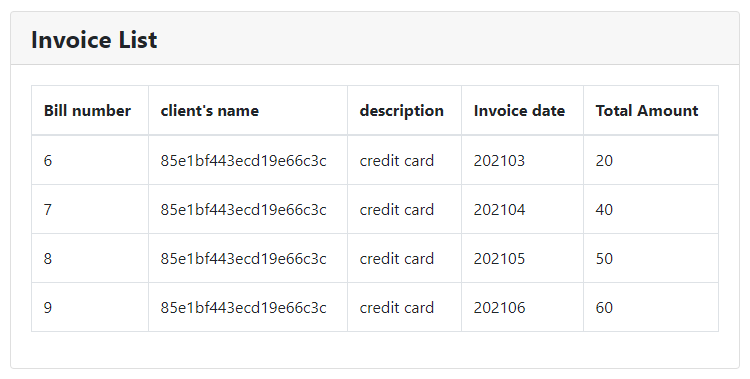
\includegraphics[height=!,width=0.8\linewidth,keepaspectratio=true]{figures/screenshot_invoicelist.png}}
    \caption{{\footnotesize Screenshot of user's invoice list}}
    \label{fig:invoicelist}
\end{figure}

\begin{figure}[htb]
    \centering
    \frame{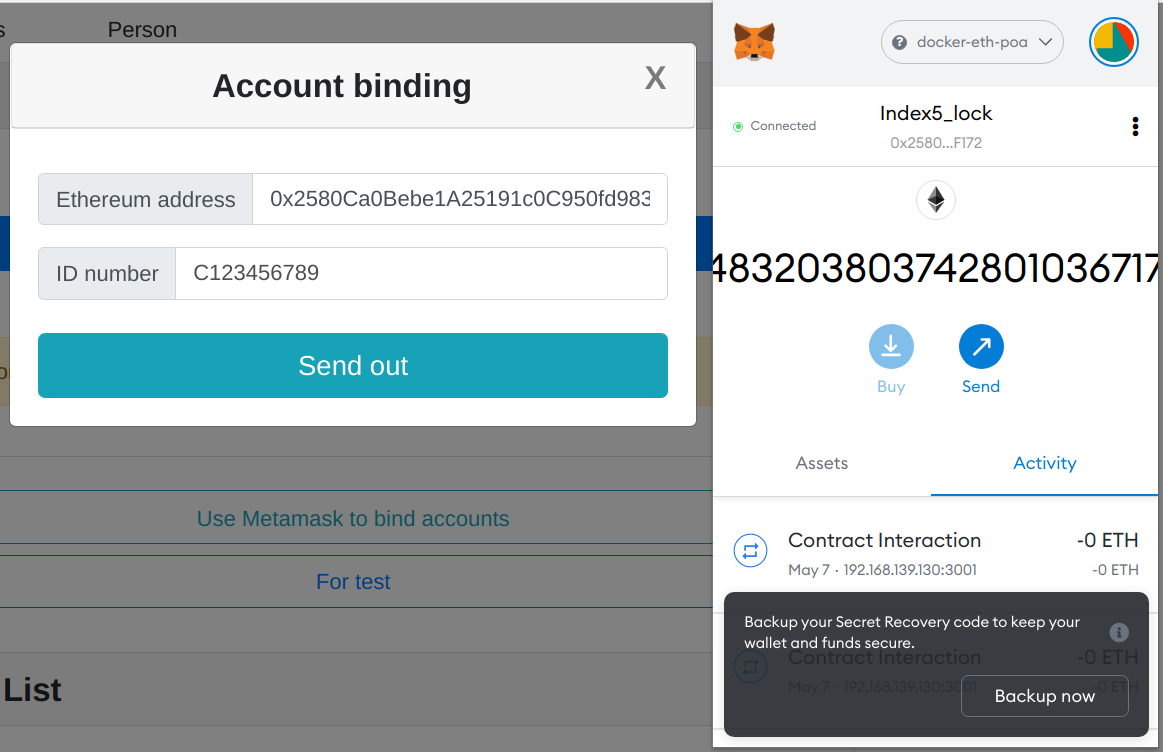
\includegraphics[height=!,width=0.8\linewidth,keepaspectratio=true]{figures/screenshot_bindconfirm.png}}
    \caption{{\footnotesize Screenshot of binding process}}
    \label{fig:bind}
\end{figure}
Besides, we define the user's bill information, the primary key of this information is his name, each user can view their own bill information as shown in Figure~\ref{fig:invoicelist}. So far, we have known two kinds of user information (balance, bill). Even if the user is not involved in a blockchain ecosystem, the user can still see their information.

\clearpage
\newpage

\section{Data sharing}

\begin{figure}[htb]
    \centering
    \frame{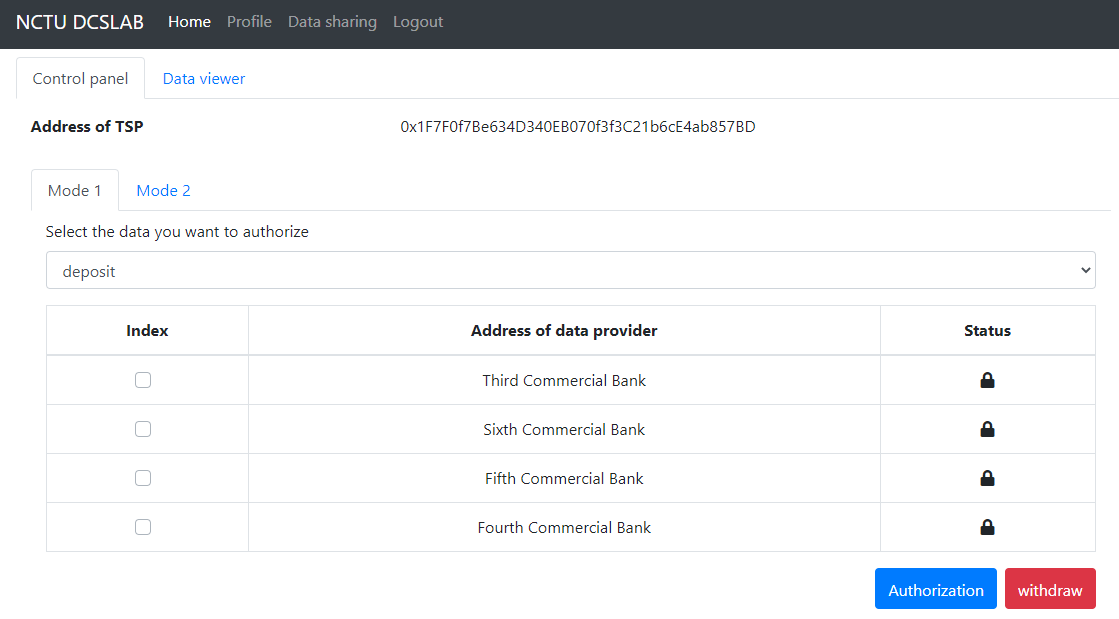
\includegraphics[height=!,width=0.8\linewidth,keepaspectratio=true]{figures/screenshot_controlpanelmode1.png}}
    \caption{{\footnotesize Screenshot of user's control panel with mode 1}}
    \label{fig:mode1}
\end{figure}

\begin{figure}[htb]
    \centering
    \frame{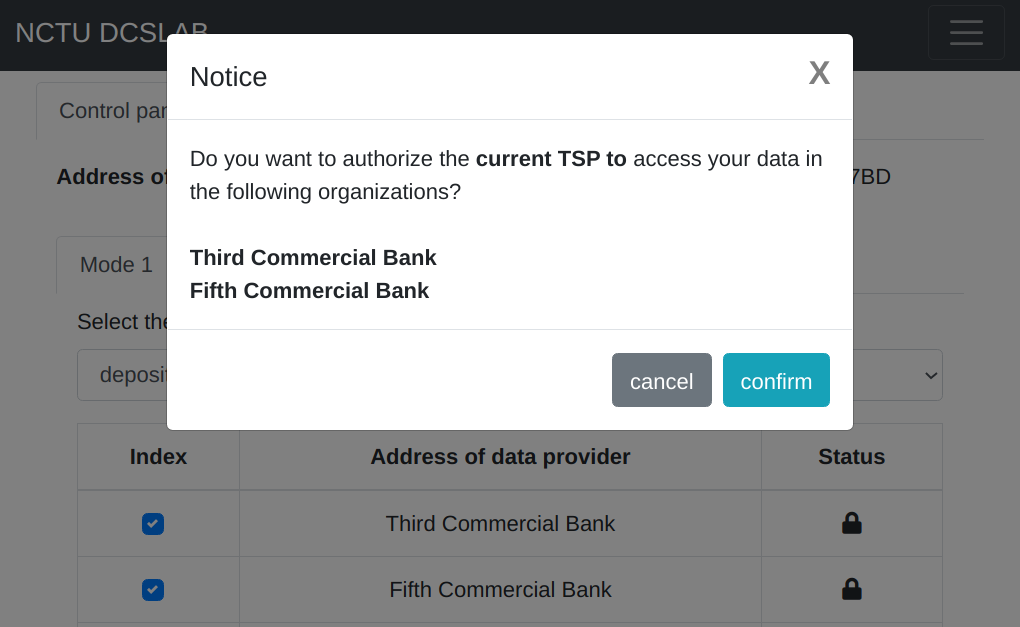
\includegraphics[height=!,width=0.8\linewidth,keepaspectratio=true]{figures/screenshot_authconfirm1.png}}
    \caption{{\footnotesize Screenshot of user's confirmation with mode 1}}
    \label{fig:mode1confirm}
\end{figure}

We provide a web-based user interface (see Figure~\ref{fig:mode1},~\ref{fig:mode2}) for users to control their data access. A user can authorize or revoke access permission at any time through the control panel of this website (see Figure~\ref{fig:mode1confirm}). Although this control panel is provided by the TSP, the TSP will not make access decisions on behalf of the user and the user can interact with web3 on the front-end side via MetaMask to connect to the specific Ethereum node.

\begin{figure}[htb]
    \centering
    \frame{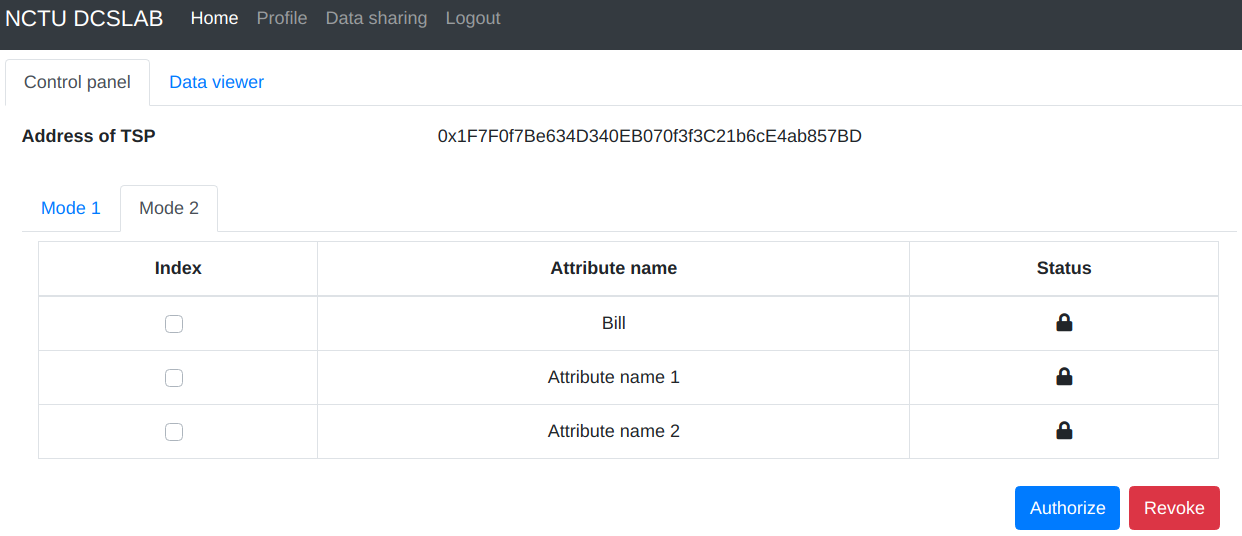
\includegraphics[height=!,width=0.9\linewidth,keepaspectratio=true]{figures/screenshot_controlpanelmode2.png}}
    \caption{{\footnotesize Screenshot of user's control panel with mode 2}}
    \label{fig:mode2}
\end{figure}

\begin{figure}[htb]
    \centering
    \frame{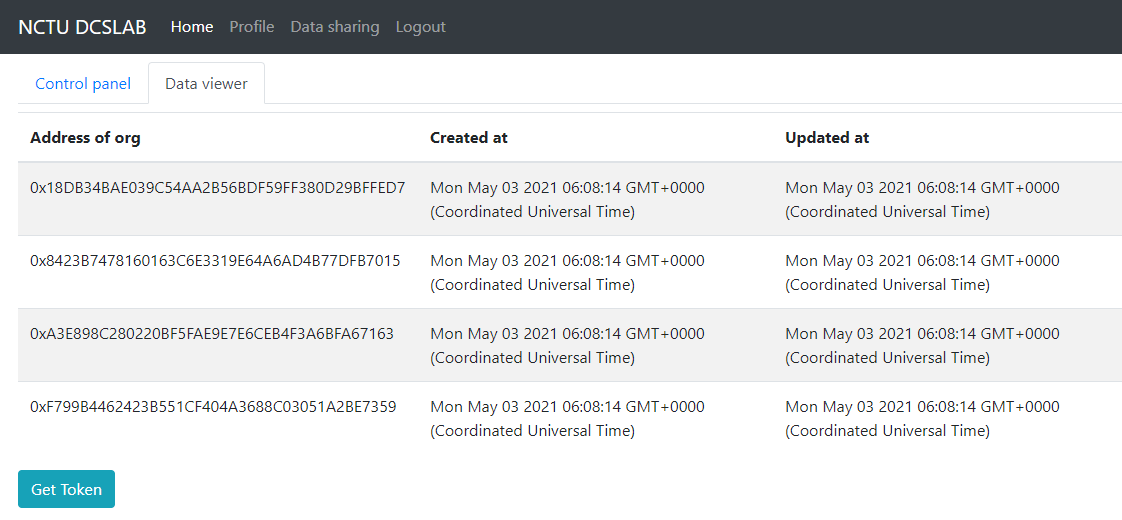
\includegraphics[height=!,width=0.9\linewidth,keepaspectratio=true]{figures/screenshot_requestJWT.png}}
    \caption{{\footnotesize Screenshot of JWTs that already stored in TSP}}
    \label{fig:sreenshotJWT}
\end{figure}
Once the access decision had been made, the user clicks on the "Get token" button to inform the TSP to request for JWTs, and then the user can view the number of JWTs that the TSP got. So that the user can trace how many JWTs are issued by banks.

\section{\textit{Org} \& \textit{TSP}}
In our implementation, an employee of the TSP and Org have to verify users' identity, so they need a web-based user interface to interact with web3 as well. The main difference lies in the architecture. As shown in the Figure~\ref{fig:verifyID}, the control panel only for employees of \(TSP\) or \(Org\).

\begin{figure}[htb]
    \centering
    \frame{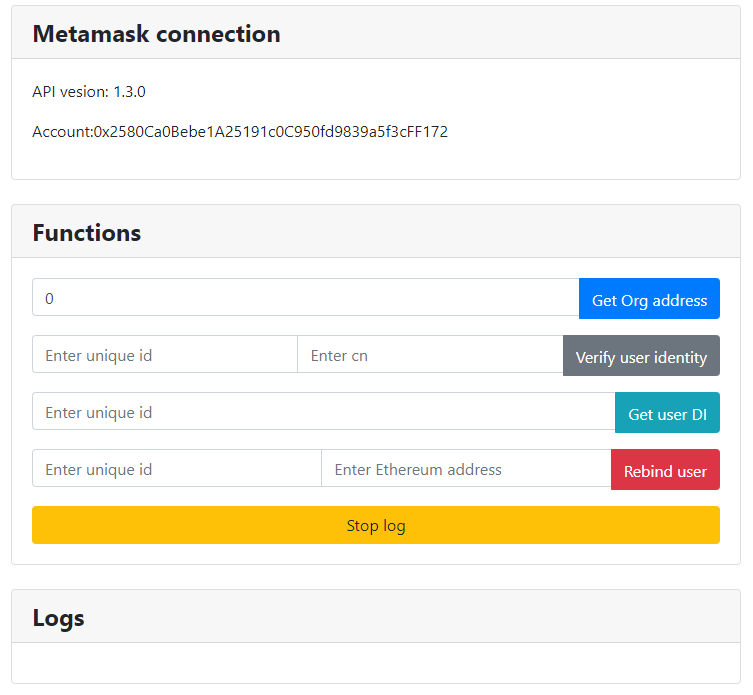
\includegraphics[height=!,width=0.75\linewidth,keepaspectratio=true]{figures/screenshot_verifyID.png}}
    \caption{{\footnotesize Screenshot of organization's administrator}}
    \label{fig:verifyID}
\end{figure}

\begin{figure}[htb]
    \centering
    \frame{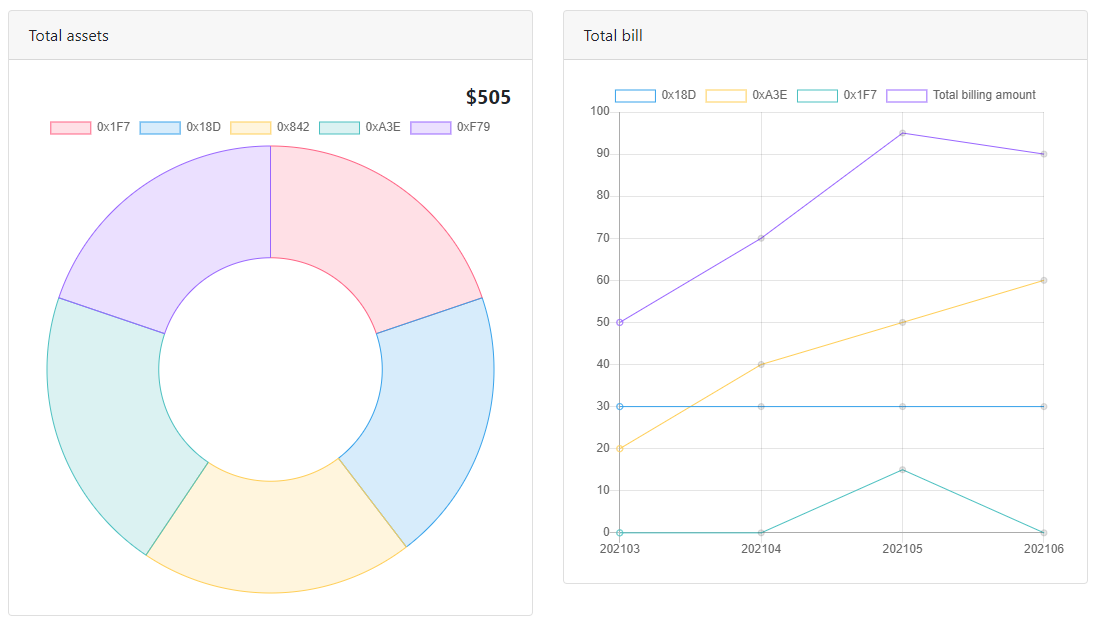
\includegraphics[height=!,width=1\linewidth,keepaspectratio=true]{figures/screenshot_tspresult.png}}
    \caption{{\footnotesize Screenshot of result that TSP generated}}
    \label{fig:result}
\end{figure}